\documentclass{article}
\usepackage[margin=2.2cm]{geometry}
\usepackage{booktabs}
\usepackage{array}
\usepackage{longtable}
\usepackage{float}
\usepackage[table]{xcolor}
\usepackage{hyperref}
\usepackage[utf8]{inputenc}
\usepackage{tikz}
\newcommand{\INF}{$\infty$}
\begin{document}
\begin{titlepage}
  \centering
  \vfill
  {\Huge Proyecto 1 - Rutas Òptimas Algoritmo de Floyd}\par
  \vspace{1cm}
  {\Large Curso: Investigación de Operaciones}\par
  {\Large Semestre: II Semestre 2025}\par
  \vfill
  {\Large Autores: Fabian Bustos - Esteban Secaida}\par
  \vspace{1cm}
  {\large Fecha: \today}\par
  \vfill
\end{titlepage}

\section*{Algoritmo de Floyd}
El algoritmo de Floyd, también conocido como Floyd--Warshall, es un método para encontrar las distancias más cortas entre todos los pares de nodos en un grafo ponderado, dirigido o no dirigido. Funciona de manera iterativa, actualizando las distancias considerando cada nodo como un posible punto intermedio entre pares de nodos.

El algoritmo fue propuesto por Robert W. Floyd en 1962, quien contribuyó significativamente al campo de la informática teórica y la optimización de algoritmos de grafos. La esencia de su trabajo reside en su simplicidad y eficacia para grafos densos.

\section*{Tablas Iniciales}
Reporte automático del algoritmo de Floyd--Warshall. Se muestran D(0) y P(0), todas las tablas intermedias D(k) y P(k) con cambios resaltados, y el resultado final.

\section*{Problema: Grafo de rutas}
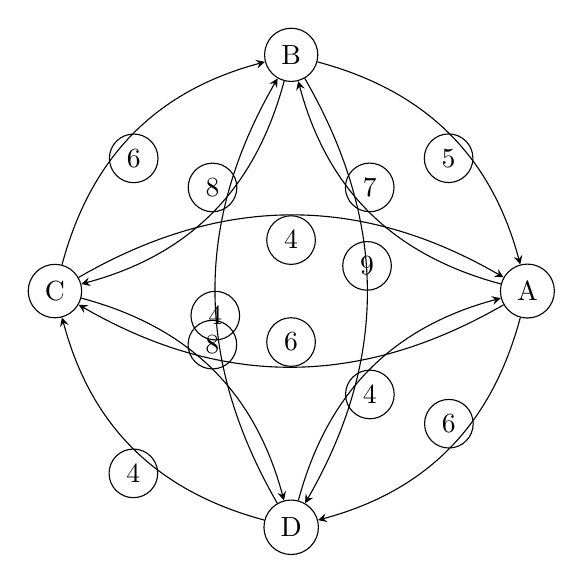
\begin{tikzpicture}[->, >=stealth, node distance=2cm, every node/.style={circle, draw}]
\node (0) at (0*360/4:3cm) {A};
\node (1) at (1*360/4:3cm) {B};
\node (2) at (2*360/4:3cm) {C};
\node (3) at (3*360/4:3cm) {D};
\draw (0) to[bend left] node[above] {7} (1);
\draw (1) to[bend left] node[below] {5} (0);
\draw (0) to[bend left] node[above] {6} (2);
\draw (2) to[bend left] node[below] {4} (0);
\draw (0) to[bend left] node[above] {6} (3);
\draw (3) to[bend left] node[below] {4} (0);
\draw (1) to[bend left] node[above] {8} (2);
\draw (2) to[bend left] node[below] {6} (1);
\draw (1) to[bend left] node[above] {9} (3);
\draw (3) to[bend left] node[below] {4} (1);
\draw (2) to[bend left] node[above] {8} (3);
\draw (3) to[bend left] node[below] {4} (2);
\end{tikzpicture}
\begin{table}[H]\centering
\caption{D(0) -- matriz de distancias inicial}
\rowcolors{2}{white}{white}
\begin{tabular}{l r r r r}
\toprule
 & \textbf{A} & \textbf{B} & \textbf{C} & \textbf{D}\\\midrule
\textbf{A} & 0 & 7 & 6 & 6 \\
\textbf{B} & 5 & 0 & 8 & 9 \\
\textbf{C} & 4 & 6 & 0 & 8 \\
\textbf{D} & 4 & 4 & 4 & 0 \\
\bottomrule
\end{tabular}
\end{table}

\begin{table}[H]\centering
\caption{P(0) -- matriz de siguiente salto inicial}
\rowcolors{2}{white}{white}
\begin{tabular}{l c c c c}
\toprule
 & \textbf{A} & \textbf{B} & \textbf{C} & \textbf{D}\\\midrule
\textbf{A} & - & B & C & D \\
\textbf{B} & A & - & C & D \\
\textbf{C} & A & B & - & D \\
\textbf{D} & A & B & C & - \\
\bottomrule
\end{tabular}
\end{table}

\section*{Tablas Intermedias}
\begin{table}[H]\centering
\caption{D(1)}
\rowcolors{2}{white}{white}
\begin{tabular}{l r r r r}
\toprule
 & \textbf{A} & \textbf{B} & \textbf{C} & \textbf{D}\\\midrule
\textbf{A} & 0 & 7 & 6 & 6 \\
\textbf{B} & 5 & 0 & 8 & 9 \\
\textbf{C} & 4 & 6 & 0 & 8 \\
\textbf{D} & 4 & 4 & 4 & 0 \\
\bottomrule
\end{tabular}
\end{table}

\begin{table}[H]\centering
\caption{P(1)}
\rowcolors{2}{white}{white}
\begin{tabular}{l c c c c}
\toprule
 & \textbf{A} & \textbf{B} & \textbf{C} & \textbf{D}\\\midrule
\textbf{A} & \cellcolor{yellow!30}A & B & C & D \\
\textbf{B} & A & \cellcolor{yellow!30}A & C & D \\
\textbf{C} & A & B & \cellcolor{yellow!30}A & D \\
\textbf{D} & A & B & C & \cellcolor{yellow!30}A \\
\bottomrule
\end{tabular}
\end{table}

\begin{table}[H]\centering
\caption{D(2)}
\rowcolors{2}{white}{white}
\begin{tabular}{l r r r r}
\toprule
 & \textbf{A} & \textbf{B} & \textbf{C} & \textbf{D}\\\midrule
\textbf{A} & 0 & 7 & 6 & 6 \\
\textbf{B} & 5 & 0 & 8 & 9 \\
\textbf{C} & 4 & 6 & 0 & 8 \\
\textbf{D} & 4 & 4 & 4 & 0 \\
\bottomrule
\end{tabular}
\end{table}

\begin{table}[H]\centering
\caption{P(2)}
\rowcolors{2}{white}{white}
\begin{tabular}{l c c c c}
\toprule
 & \textbf{A} & \textbf{B} & \textbf{C} & \textbf{D}\\\midrule
\textbf{A} & A & B & C & D \\
\textbf{B} & A & A & C & D \\
\textbf{C} & A & B & A & D \\
\textbf{D} & A & B & C & A \\
\bottomrule
\end{tabular}
\end{table}

\begin{table}[H]\centering
\caption{D(3)}
\rowcolors{2}{white}{white}
\begin{tabular}{l r r r r}
\toprule
 & \textbf{A} & \textbf{B} & \textbf{C} & \textbf{D}\\\midrule
\textbf{A} & 0 & 7 & 6 & 6 \\
\textbf{B} & 5 & 0 & 8 & 9 \\
\textbf{C} & 4 & 6 & 0 & 8 \\
\textbf{D} & 4 & 4 & 4 & 0 \\
\bottomrule
\end{tabular}
\end{table}

\begin{table}[H]\centering
\caption{P(3)}
\rowcolors{2}{white}{white}
\begin{tabular}{l c c c c}
\toprule
 & \textbf{A} & \textbf{B} & \textbf{C} & \textbf{D}\\\midrule
\textbf{A} & A & B & C & D \\
\textbf{B} & A & A & C & D \\
\textbf{C} & A & B & A & D \\
\textbf{D} & A & B & C & A \\
\bottomrule
\end{tabular}
\end{table}

\begin{table}[H]\centering
\caption{D(4)}
\rowcolors{2}{white}{white}
\begin{tabular}{l r r r r}
\toprule
 & \textbf{A} & \textbf{B} & \textbf{C} & \textbf{D}\\\midrule
\textbf{A} & 0 & 7 & 6 & 6 \\
\textbf{B} & 5 & 0 & 8 & 9 \\
\textbf{C} & 4 & 6 & 0 & 8 \\
\textbf{D} & 4 & 4 & 4 & 0 \\
\bottomrule
\end{tabular}
\end{table}

\begin{table}[H]\centering
\caption{P(4)}
\rowcolors{2}{white}{white}
\begin{tabular}{l c c c c}
\toprule
 & \textbf{A} & \textbf{B} & \textbf{C} & \textbf{D}\\\midrule
\textbf{A} & A & B & C & D \\
\textbf{B} & A & A & C & D \\
\textbf{C} & A & B & A & D \\
\textbf{D} & A & B & C & A \\
\bottomrule
\end{tabular}
\end{table}

\section*{Distancias y rutas óptimas}
\begin{table}[H]\centering
\caption{D(final)}
\rowcolors{2}{white}{white}
\begin{tabular}{l r r r r}
\toprule
 & \textbf{A} & \textbf{B} & \textbf{C} & \textbf{D}\\\midrule
\textbf{A} & 0 & 7 & 6 & 6 \\
\textbf{B} & 5 & 0 & 8 & 9 \\
\textbf{C} & 4 & 6 & 0 & 8 \\
\textbf{D} & 4 & 4 & 4 & 0 \\
\bottomrule
\end{tabular}
\end{table}

\begin{table}[H]\centering
\caption{P(final)}
\rowcolors{2}{white}{white}
\begin{tabular}{l c c c c}
\toprule
 & \textbf{A} & \textbf{B} & \textbf{C} & \textbf{D}\\\midrule
\textbf{A} & A & B & C & D \\
\textbf{B} & A & A & C & D \\
\textbf{C} & A & B & A & D \\
\textbf{D} & A & B & C & A \\
\bottomrule
\end{tabular}
\end{table}

\subsection*{Listado de rutas (todas las parejas i $\neq$ j)}
\begin{longtable}{llp{0.65\textwidth}}
\toprule
\textbf{Origen} & \textbf{Destino} & \textbf{Ruta óptima (con saltos)}\\\midrule
A & B & A → B (distancia = 7)\\
A & C & A → C (distancia = 6)\\
A & D & A → D (distancia = 6)\\
B & A & B → A (distancia = 5)\\
B & C & B → C (distancia = 8)\\
B & D & B → D (distancia = 9)\\
C & A & C → A (distancia = 4)\\
C & B & C → B (distancia = 6)\\
C & D & C → D (distancia = 8)\\
D & A & D → A (distancia = 4)\\
D & B & D → B (distancia = 4)\\
D & C & D → C (distancia = 4)\\
\bottomrule
\end{longtable}
\end{document}